% !TeX encoding = UTF-8
% !TeX spellcheck = en_US
\section{Case Studies}
\label{sec:case_studies}

This section presents two case studies in simulation to demonstrate the design of linear and nonlinear MPCs. The objective here is to demonstrate how the package syntax facilitates the implementation and testing of predictive controllers and state estimators. The package manager of Julia simplifies the installation of \texttt{ModelPredictiveControl.jl}:
\begin{minted}{julia}
using Pkg; Pkg.add("ModelPredictiveControl")
\end{minted}
The first example details how to apply an MPC on a plant at each discrete time step. The second uses higher-level functionalities to quickly simulate closed-loop systems.

\subsection{Linear Design: Continuously Stirred Tank Reactor}

\subsubsection{Linear Model}

The example considers a continuously stirred tank reactor (CSTR) with a cold and hot water intakes, fed at a respective flow rate of $u_c$ and $u_h$. The manipulated input vector is thus $\mathbf{u} = [\begin{smallmatrix}u_c & u_h\end{smallmatrix}]^\intercal$. The liquid level $y_L$ and temperature $y_T$ constitute the measured output vector $\mathbf{y} = [\begin{smallmatrix}y_L & y_T\end{smallmatrix}]^\intercal$. \cref{fig:cstr} presents schematically the case study process.

\begin{figure}
    \centering
    \caption{CSTR process.}
    \begin{tikzpicture}[scale=1]
       
\fill[blue!10](0.0,0) rectangle (1.5,1.5);
\fill[blue!10](1.5,0) rectangle (1.8,0.3);

\draw[blue!30] (0.0, 1.5) -- (1.5,1.5);

\draw[<-,semithick] (0.45,0.75) arc (180:-150:0.3 and 0.3);

\draw[line width=2.2] (0, 2) -- (0, 0) -- (1.8,0);
\draw[line width=2.2] (1.8,0.3) -- (1.5,0.3) -- (1.5,2);

\pic[scale=0.6] (T) at (-0.6,1.20) {instrument=$y_T$};
\pic[scale=0.6] (L) at (+2.1,1.50) {instrument=$y_L$};

\draw [latex-latex] (1.675,1.25) -- (1.676,1.75);

\draw (T-right) -- ++(+0.6,0);
\draw (L-left)  -- ++(-0.3,0);

\pic [blue] (VC)    at (-0.6, 2.25) {valve=secondary};
\pic [blue] (VCact) at (-0.6, 2.25) {actuator};
\pic [red]  (VH)    at (2.1, 2.25) {valve=secondary};
\pic [red]  (VHact) at (2.1, 2.25) {actuator};

\draw[main stream, blue] (VC-right) -- node[above, black]{$u_c$} (0.5, 2.25) -| ++(0,-0.5);
\draw[main stream, red]  (VH-left)  -- node[above, black]{$u_h$} (1.0, 2.25) -| ++(0,-0.5);
\draw[main stream, blue] (-1.3, 2.25) -- (VC-left);
\draw[main stream, red]  (+2.8, 2.25) -- (VH-right);
\draw[main stream] (1.8,0.15) -- ++(0.5, 0);

\end{tikzpicture}
    \label{fig:cstr}
\end{figure}

At the steady-state operating point $u_c=u_h=20$, $y_L=50$, and $y_T=30$, the following linear model accurately describes the plant dynamics:
\begin{equation}
\mathbf{G}(s) = \frac{\mathbf{y}(s)}{\mathbf{u}(s)} =
\begin{bmatrix}
    \frac{1.90}{18s+1} & \frac{1.90}{18s+1} \\[3pt]
    \frac{-0.74}{8s+1} & \frac{0.74}{8s+1}
\end{bmatrix}
\end{equation}
The syntax to construct a linear model with a sample time of $\SI{2}{\second}$ is:
\begin{minted}{julia}
using ModelPredictiveControl, ControlSystemsBase
G = [ tf(1.90, [18, 1]) tf(1.90, [18, 1]);
      tf(-0.74,[8, 1])  tf(0.74, [8, 1]) ]
model = setop!(LinModel(G, 2.0); uop=[20,20], yop=[50,30])
vu, vy = ["\$u_c\$", "\$u_h\$"], ["\$y_L\$", "\$y_T\$"]
model = setname!(model; u=vu, y=vy)
\end{minted}
\spacerepl
\begin{minted}{julia-repl}
LinModel with a sample time Ts = 2.0 s and:
 2 manipulated inputs u
 2 states x
 2 outputs y
 0 measured disturbances d
\end{minted}
The \texttt{model} object is used for two purposes : to construct our controller and as a plant simulator to test the design. The \texttt{setname!} function customizes the $y$-axis labels in the plots.

\subsubsection{Linear Model Predictive Controller}

The objective is to maintain both the water temperature and level at their respective setpoints while constraining the level above 45:
\begin{minted}{julia}
mpc = setconstraint!(LinMPC(model), ymin=[45, -Inf])
\end{minted}
\spacerepl
\begin{minted}{julia-repl}
LinMPC controller with a sample time Ts = 2.0 s, OSQP optimizer, 
SteadyKalmanFilter estimator and:
 10 prediction steps Hp
  2 control steps Hc
  1 slack variable ϵ (control constraints)
  2 manipulated inputs u (0 integrating states)
  4 estimated states x̂
  2 measured outputs ym (2 integrating states)
  0 unmeasured outputs yu
  0 measured disturbances d
\end{minted}
By default, \texttt{LinMPC} controllers use \texttt{OSQP.jl} \citep{osqp} to solve the problem, soft constraints on output predictions $\mathbf{\hat y}$ to ensure feasibility, and a \texttt{SteadyKalmanFilter} to estimate the plant states. The default predictive and control horizons are $H_p = 10 + n_k$ and $H_c = 2$, respectively, where $n_k$ is the number of delays in the linear model. The $H_c$ value is small by default to reduce the computational burden and the aggressiveness \citep{mpcHcAnalysis}. An attentive reader will also notice that the Kalman filter estimates two additional states compared to the plant model. These are the integrating states for the unmeasured plant disturbances, and they are automatically added at the model output $\mathbf{y}$ by default if observability is preserved.

On a side note, an internal model structure could have been used with \texttt{estim = InternalModel(model)} and \texttt{mpc = setconstraint!(LinMPC(estim); ymin=[45, -Inf])}, as an alternative to state estimator. It was tested on this example and it gave similar results.

Before closing the loop, the actual plant input $\mathbf{u}$ and measurement $\mathbf{y^m}$ should initialize the estimates $\mathbf{\hat{x}}$ at the steady-state solution that leads to $\mathbf{\hat{y}^m}(0)=\mathbf{y^m}(0)$. This approach results in a bumpless transfer, especially with estimators in the predictor form. The \texttt{initstate!} function finds this solution for \texttt{LinModel}. Since the plant is the model here, its output initializes the states. \texttt{LinModel} objects are callable for this purpose. Once done, imposing step changes on the setpoint \texttt{ry} and on a load disturbance \texttt{ul} tests the closed-loop performance of \texttt{mpc}:
\begin{minted}{julia}
function test_mpc(mpc, plant)
    plant.x0 .= 0; y = plant() # or evaloutput(plant)
    initstate!(mpc, plant.uop, y)
    N = 75; ry = [50, 30]; ul = 0
    U, Y, Ry = zeros(2, N), zeros(2, N), zeros(2, N)
    for i = 1:N
        i == 26 && (ry = [48, 35])
        i == 51 && (ul = -10)
        y = plant() # simulated measurements
        u = mpc(ry) # or moveinput!(mpc, ry)
        U[:,i], Y[:,i], Ry[:,i] = u, y, ry
        updatestate!(mpc, u, y) # update mpc estimate
        updatestate!(plant, u+[0,ul]) # update simulator
    end
    return U, Y, Ry
end
U_data, Y_data, Ry_data = test_mpc(mpc, model)
\end{minted}
Calling \texttt{LinMPC} instances computes and returns $\mathbf{u}(k)$. It is worth mentioning that additional information like the optimal output predictions $\mathbf{\hat{Y}}$ can be retrieved by calling \texttt{getinfo} after solving the problem. Also, updating the internal states of \texttt{mpc} prepares the object for the \emph{next} time step. That is why the call is made at the end of the \texttt{for} loop. The same logic applies for \texttt{plant}. Lastly, the package implements a \texttt{Plots.jl} recipe \citep{plots} to quickly visualize the results:
\begin{minted}{julia}
res = SimResult(mpc, U_data, Y_data; Ry_data)
using Plots; plot(res)
\end{minted}
\cref{fig:plot_LinMPC1} shows that the controller violates the constraints around 110 s because of the disturbance. Adding feedforward compensation can mitigate this.

\begin{figure}[ht]
    \centering
    \caption{CSTR closed-loop simulation (MPC).}
    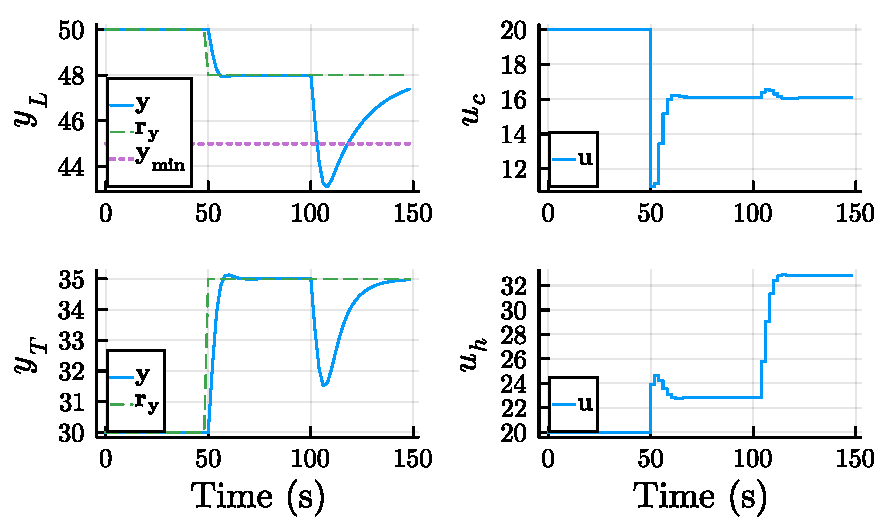
\includegraphics[width=0.5\columnwidth]{fig/plot_LinMPC1.pdf}
    \label{fig:plot_LinMPC1}
\end{figure}

\subsubsection{Feedforward Compensation}

Suppose that the load disturbance $u_l$ is in fact caused by a separate hot water pipe that discharges into the tank. Measuring this flow rate allows us to incorporate feedforward compensation with $\mathbf{d}=u_l$. The new plant model is:

\begin{minted}{julia}
model_d = LinModel([G G[1:2, 2]], 2.0; i_d=[3])
model_d = setop!(model_d; uop=[20,20], yop=[50,30], dop=[20])
model_d = setname!(model_d; u=vu, y=vy, d=["\$u_l\$"])
\end{minted}
\spacerepl
\begin{minted}{julia-repl}
Discrete-time linear model with a sample time Ts = 2.0 s and:
 2 manipulated inputs u
 4 states x
 2 outputs y
 1 measured disturbances d
\end{minted}
The simulation needs a new \texttt{LinMPC} object based on \texttt{model\_d} and a new test function that explicitly employs the current disturbance measurement:
\begin{minted}{julia}
mpc_d = setconstraint!(LinMPC(model_d), ymin=[45, -Inf])
function test_mpc_d(mpc_d, plant)
    plant.x0 .= 0; y = plant(); d = [20]
    initstate!(mpc_d, plant.uop, y, d)
    N = 75; ry = [50, 30]; ul = 0
    U, Y, Ry = zeros(2, N), zeros(2, N), zeros(2, N)
    for i = 1:N
        i == 26 && (ry = [48, 35])
        i == 51 && (ul = -10)
        y, d = plant(), [20+ul] # simulated measurements
        u = mpc_d(ry, d) # d in arguments
        U[:,i], Y[:,i], Ry[:,i] = u, y, ry
        updatestate!(mpc_d, u, y, d) # d in arguments
        updatestate!(plant, u+[0,ul])
    end
    return U, Y, Ry
end
U_data, Y_data, Ry_data = test_mpc_d(mpc_d, model)
res = SimResult(mpc, U_data, Y_data; Ry_data)
plot(res)
\end{minted}
\cref{fig:plot_LinMPC2} shows that the feedforward compensation handles the disturbance without violating the constraint. Note that measured disturbances are assumed constant in the future by default but custom $\mathbf{\hat{D}}$ predictions are possible. The same applies for the setpoints $\mathbf{\hat{R}_y}$ and $\mathbf{\hat{R}_u}$. For instance, the stochastic predictions of an \texttt{InternalModel} can generate these vectors.

\begin{figure}[ht]
    \centering
    \caption{CSTR closed-loop simulation with feedforward (MPC).}
    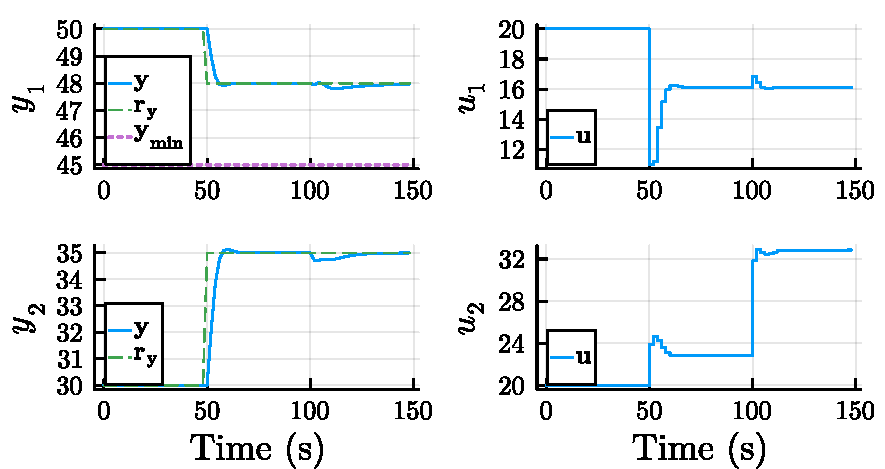
\includegraphics[width=0.5\columnwidth]{fig/plot_LinMPC2.pdf}
    \label{fig:plot_LinMPC2}
\end{figure}

\subsection{Nonlinear Design : Inverted Pendulum}
\label{sec.nonlinear_design}

\subsubsection{Nonlinear Model}

\begin{figure}
    \centering
    \caption{Inverted pendulum.}
    \begin{tikzpicture}[scale=1]
       
\fill (-0.85,-0.2) rectangle (0.85,0.2);
\draw (-1.5,0) -- (1.5,0) node[above, very near start]{$\tau$};
\draw[fill=white] (0,0) circle (0.75);


\fill (0,0) circle (0.15);

\draw[line width=2.2] (0,0) -- (0,1.3);
\draw[densely dotted, gray] (0,0) -- (0,-0.5);
\draw[gray, <-] (0,0.3) arc [start angle=90, end angle=-90, radius=0.3];
\node[gray] at (0.5, 0.0) {$\theta$};

\node[black] at (-0.35, 0.0) {$K$};

\filldraw (0, 1.6) circle (0.3) node[white]{$m$};

\draw [Stealth-Stealth] (1.2, 0) -- node[fill=white]{$L$} (1.2, 1.6);
\draw (1.15, 1.6) -- (1.25, 1.6);

\end{tikzpicture}
    \label{fig:pendulum}
\end{figure}

For this case study, the goal is to control the angular position $\theta$ of a pendulum attached to a motor, thus $\mathbf{y} = \theta$. The manipulated input is the motor torque $\mathbf{u} = \tau$ in \si{\newton\meter}. \cref{fig:pendulum} depicts the system. The model is:
\begin{subequations}
\begin{align}
\dot{\theta}(t) &= \omega(t) \\
\dot{\omega}(t) &= -\frac{g}{L}\sin\big(\theta(t)\big) -\frac{K}{m}\omega(t) + \frac{1}{m L^2}\tau(t) \label{eq.pendulum_speed}
\end{align}
\end{subequations}
in which $g$ is the gravitational acceleration in \si{\meter\per\second\squared}, $L$, the pendulum length in \si{\meter}, $K$, the friction coefficient at the pivot point in \si{\kilogram\per\second}, and $m$, the mass attached at the end of the pendulum in \si{\kilogram}. By default, the \texttt{NonLinModel} constructor assumes continuous-time equations and discretizes them with Runge-Kutta:
\begin{minted}{julia}
using ModelPredictiveControl
function pendulum!(ẋ, x, u, par)
    g, L, K, m = par     # [m/s²], [m], [kg/s], [kg]
    θ, ω = x[1], x[2]    # [rad], [rad/s]
    τ = u[1]             # [Nm]
    ẋ[1] = ω
    ẋ[2] = -g/L*sin(θ) - K/m*ω + τ/m/L^2
    return nothing
end
const par = (9.8, 0.4, 1.2, 0.3)
f!(ẋ, x, u, _ ) = pendulum!(ẋ, x, u, par)
h!(y, x, _ ) = (y[1] = 180/π*x[1])   # [°]
nu = 1; nx = 2; ny = 1; Ts = 0.1
model = NonLinModel(f!, h!, Ts, nu, nx, ny)
vu = ["\$τ\$ (Nm)"]
vx = ["\$θ\$ (rad)", "\$ω\$ (rad/s)"]
vy = ["\$θ\$ (°)"]
model = setname!(model; u=vu, x=vx, y=vy)
\end{minted}
\spacerepl
\begin{minted}{julia-repl}
NonLinModel with a sample time Ts = 0.1 s, RungeKutta solver and:
 1 manipulated inputs u
 2 states x
 1 outputs y
 0 measured disturbances d
\end{minted}

The output function $\mathbf{h}$ converts the $\theta$ angle to degrees. The plant model relies on mutating state-space functions to reduce the memory allocations and the computational burden as well. The more intuitive non-mutating syntax can still be used by providing functions with one less argument, e.g.: \texttt{f(x,u,d)=x+u+d} and \texttt{h(x,d)=x+d}.

\subsubsection{Nonlinear State Estimator}

The state estimates of an \texttt{UnscentedKalmanFilter} will feed the controller:
\begin{minted}{julia}
σQ = [0.1, 0.5]; σR=[0.5]; nint_u=[1]; σQint_u=[0.1]
estim = UnscentedKalmanFilter(model; σQ, σR, nint_u, σQint_u)
\end{minted}
\spacerepl
\begin{minted}{julia-repl}
UnscentedKalmanFilter estimator with a sample time Ts = 0.1 s, NonLinModel and:
 1 manipulated inputs u (1 integrating states)
 3 states x̂
 1 measured outputs ym (0 integrating states)
 0 unmeasured outputs yu
 0 measured disturbances d
\end{minted}
The vectors \texttt{σQ} and \texttt{σR} are the standard deviations of the process and sensor noises, respectively. The value for the velocity $\omega$ is higher here (\texttt{σQ} second value) since \eqref{eq.pendulum_speed} includes an uncertain parameter: the friction coefficient $K$. Also, the argument \texttt{nint\_u} explicitly adds one integrating state at the model input, the motor torque $\tau$, with an associated standard deviation \texttt{σQint\_u} of $\SI{0.1}{\newton\meter}$. Custom models for the unmeasured disturbances will be added in a future release (other than integrators). The estimator tuning is tested on a plant with a \SI{25}{\percent} larger friction coefficient $K$: 
\begin{minted}{julia}
par_plant = (par[1], par[2], 1.25*par[3], par[4])
f_plant!(ẋ, x, u, _) = pendulum!(ẋ, x, u, par_plant)
plant = NonLinModel(f_plant!, h!, Ts, nu, nx, ny)
N = 35; u = [0.5]; y_noise = [0.5]
res = sim!(estim, N, u; plant, y_noise)
using Plots; plot(res, plotu=false, plotxwithx̂=true)
\end{minted}
\cref{fig:plot_NonLinMPC1} indicates that the Kalman filter performance seems sufficient for control. The estimate $\hat{x}_3$ is the integrating state on the torque $\tau$ that compensates for static errors. 

\begin{figure}[ht]
    \centering
    \caption{Pendulum state estimation.}
    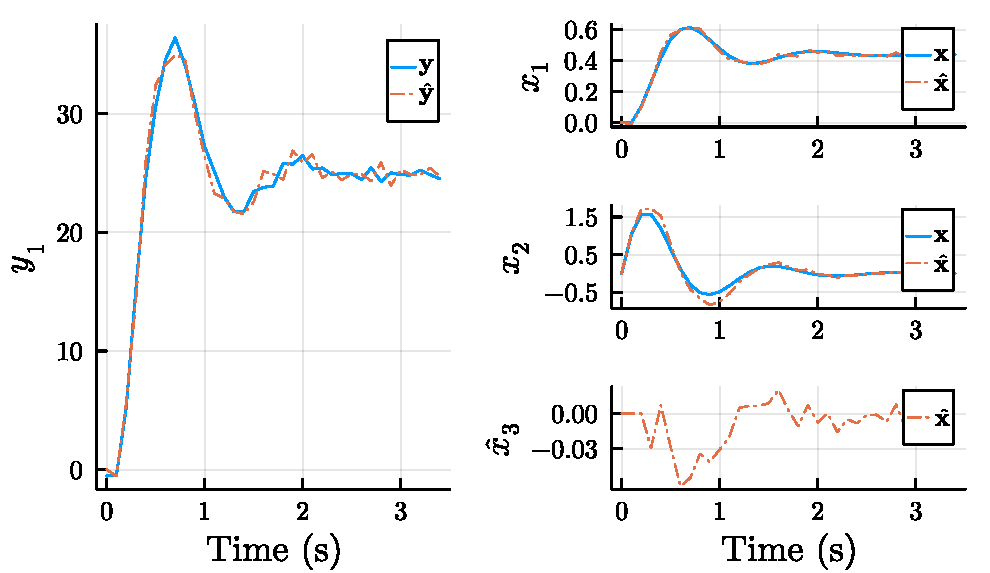
\includegraphics[width=0.5\columnwidth]{fig/plot_NonLinMPC1.pdf}
    \label{fig:plot_NonLinMPC1}
\end{figure}

\subsubsection{Nonlinear Model Predictive Controller (NMPC)}

As the motor torque is limited to \num{-1.5} to \SI{1.5}{\newton\meter}, the input constraints are incorporated to a \texttt{NonLinMPC} object:
\begin{minted}{julia}
Hp, Hc, Mwt, Nwt, Cwt = 20, 2, [0.5], [2.5], Inf
nmpc = NonLinMPC(estim; Hp, Hc, Mwt, Nwt, Cwt)
umin, umax = [-1.5], [+1.5]
nmpc = setconstraint!(nmpc; umin, umax)
\end{minted}
\spacerepl
\begin{minted}{julia-repl}
NonLinMPC controller with a sample time Ts = 0.1 s, Ipopt optimizer, 
UnscentedKalmanFilter estimator and:
 20 prediction steps Hp
  2 control steps Hc
  0 slack variable ϵ (control constraints)
  1 manipulated inputs u (1 integrating states)
  3 estimated states x̂
  1 measured outputs ym (0 integrating states)
  0 unmeasured outputs yu
  0 measured disturbances d
\end{minted}
The keyword arguments \texttt{Mwt} and \texttt{Nwt} are the output setpoint tracking and move suppression weights, respectively. The option \texttt{Cwt=Inf} disables the slack variable $\epsilon$. An angular setpoint of \SI{180}{\degree} (inverted position) tests \texttt{mpc} performance on the plant:
\begin{minted}{julia}
x_0 = [0, 0]; x̂_0 = [0, 0, 0]; ry = [180]
res_ry = sim!(nmpc, N, ry; plant, x_0, x̂_0)
plot(res_ry)
\end{minted}
The result in \cref{fig:plot_NonLinMPC2} suggests that the controller is robust enough to variations on the $K$ coefficient. Starting from this inverted position, \cref{fig:plot_NonLinMPC3} shows the closed-loop response to a step disturbances of \SI{10}{\degree} is satisfactory:
\begin{minted}{julia}
x_0 = [π, 0]; x̂_0 = [π, 0, 0]; y_step = [10]
res_yd = sim!(nmpc, N, [180.0]; plant, x_0, x̂_0, y_step)
plot(res_yd)
\end{minted}
The next section presents an economic predictive controller on the pendulum.

\begin{figure}[t]
    \centering
    \caption{Pendulum output setpoint tracking (NMPC).}
    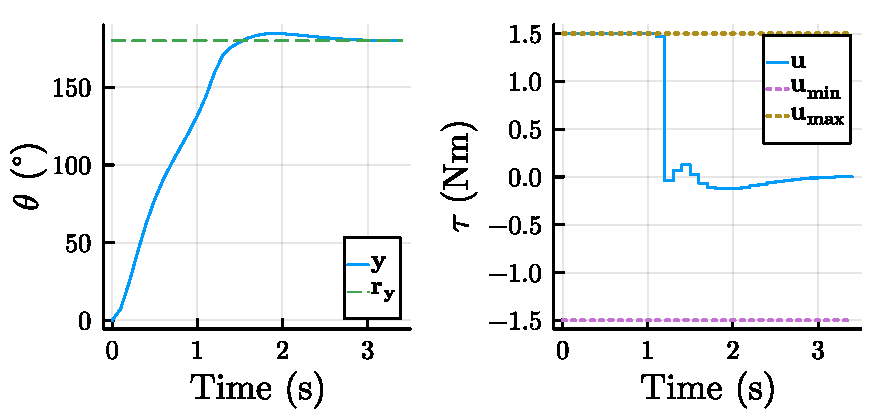
\includegraphics[width=0.5\columnwidth]{fig/plot_NonLinMPC2.pdf}
    \label{fig:plot_NonLinMPC2}
\end{figure}

\begin{figure}[t]
    \centering
    \caption{Pendulum output disturbance rejection (NMPC).}
    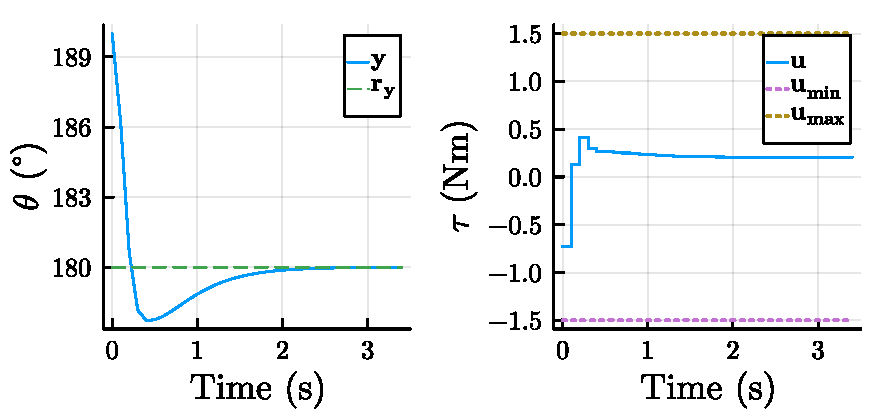
\includegraphics[width=0.5\columnwidth]{fig/plot_NonLinMPC3.pdf}
    \label{fig:plot_NonLinMPC3}
\end{figure}

\subsubsection{Economic model predictive control (EMPC)}

For this case study, the controller will aim to reduce the energy consumed by the motor. The power in watt transmitted by the motor to the pendulum is:
\begin{equation}
P(t) = \tau(t) \omega(t) 
\end{equation}
Thus, the work in joule done by the motor from $t_0$ to $t_{end}$ is:
\begin{equation}
W = \int_{t_0}^{t_{end}} P(t) \mathrm{d}t 
\end{equation}
With the sampling time $T_s$ in second and the prediction horizon $H_p$ in time steps, computing the integral with the left-endpoint rectangle method and defining the limits as $t_0=k$ and $t_{end} = (k + H_p) T_s$ give:
\begin{equation}\label{eq:pendulum_W}
W \approx T_s \sum_{j = 0}^{H_p - 1} \tau(k+j) \omega(k+j) 
\end{equation}

The objective will now include an additive term that penalizes the work done by the motor $W$ to reduce the energy consumption. Notice that \eqref{eq:pendulum_W} is a function of the manipulated input $\tau$ and the angular speed $\omega$, a state that is not measured (only the angle $\theta$ is measured here). As the arguments of the economic function $J_E$ in \eqref{eq:J_NMPC} do not include the states, the speed is now defined as an unmeasured output to design a Kalman filter similar to the previous one ($\mathbf{y^m} = \theta$ and $\mathbf{y^u} = \omega$): 

\begin{minted}{julia}
h2!(y, x, _ ) = (y[1] = 180/π*x[1]; y[2]=x[2])
nu, nx, ny = 1, 2, 2
model2 = NonLinModel(f!      , h2!, Ts, nu, nx, ny)
plant2 = NonLinModel(f_plant!, h2!, Ts, nu, nx, ny)
model2 = setname!(model2, u=vu, x=vx, y=[vy; vx[2]])
plant2 = setname!(plant2, u=vu, x=vx, y=[vy; vx[2]])
estim2 = UnscentedKalmanFilter(model2; σQ, σR, nint_u, σQint_u, i_ym=[1])
\end{minted}
The \texttt{plant2} object based on \texttt{h2!} is also required since \texttt{sim!} expects that the plant output vector $\mathbf{y}$ corresponds to the controller model output vector. Now, these lines define the $J_E$ function and the controller:
\begin{minted}{julia}
function JE(UE, ŶE, _ )
    τ, ω = UE[1:end-1], ŶE[2:2:end-1]
    return Ts*sum(τ.*ω)
end
Mwt2, Ewt = [Mwt; 0.0], 3.5e3
empc = NonLinMPC(estim2; Hp, Hc, Nwt, Mwt=Mwt2, Cwt, JE, Ewt)
empc = setconstraint!(empc; umin, umax)
\end{minted}
\spacerepl
\begin{minted}{julia-repl}
NonLinMPC controller with a sample time Ts = 0.1 s, Ipopt optimizer, 
UnscentedKalmanFilter estimator and:
 20 prediction steps Hp
  2 control steps Hc
  0 slack variable ϵ (control constraints)
  1 manipulated inputs u (1 integrating states)
  3 estimated states x̂
  1 measured outputs ym (0 integrating states)
  1 unmeasured outputs yu
  0 measured disturbances d
\end{minted}

The keyword argument \texttt{Ewt} is the $E$ weight in \eqref{eq:J_NMPC}. The economic term must be large enough to be significant but a too high value can lead to a static error on the angle setpoint. The second element of \texttt{Mwt2} is zero since the speed $\omega$ is not requested to track a setpoint. \cref{fig:plot_EconomMPC1} shows that closed-loop response to a \SI{180}{\degree} setpoint is similar:
\begin{minted}{julia}
x_0 = [0, 0]; x̂_0 = [0, 0, 0]; ry = [180; 0]
res2_ry = sim!(empc, N, ry; plant=plant2, x_0, x̂_0)
plot(res2_ry, ploty=[1])
\end{minted}
and the energy consumption is slightly lower:
\begin{minted}{julia}
function calcW(res)
    τ, ω = res.U_data[1, 1:end-1], res.X_data[2, 1:end-1]
    return Ts*sum(τ.*ω)
end
Dict(:W_nmpc => calcW(res_ry), :W_empc => calcW(res2_ry))
\end{minted}
\spacerepl
\begin{minted}{julia-repl}
Dict{Symbol, Float64} with 2 entries:
  :W_empc => 3.89437
  :W_nmpc => 3.91597
\end{minted}
Also, for a \SI{10}{\degree} step disturbance (results depicted in \cref{fig:plot_EconomMPC2}):
\begin{minted}{julia}
x_0 = [π, 0]; x̂_0 = [π, 0, 0]; y_step = [10; 0]
res2_yd = sim!(empc, N, ry; plant=plant2, x_0, x̂_0, y_step)
plot(res2_yd, ploty=[1])
\end{minted}
the new controller is able to recuperate more energy from the pendulum (i.e. negative work):
\begin{minted}{julia}
Dict(:W_nmpc => calcW(res_yd), :W_empc => calcW(res2_yd))
\end{minted}
\spacerepl
\begin{minted}{julia-repl}
Dict{Symbol, Float64} with 2 entries:
  :W_empc => -0.149044
  :W_nmpc => -0.112247
\end{minted}
Of course, this gain is only exploitable if the motor electronic includes some kind of regenerative circuitry.

\begin{figure}[ht]
    \centering
    \caption{Pendulum output setpoint tracking (EMPC).}
    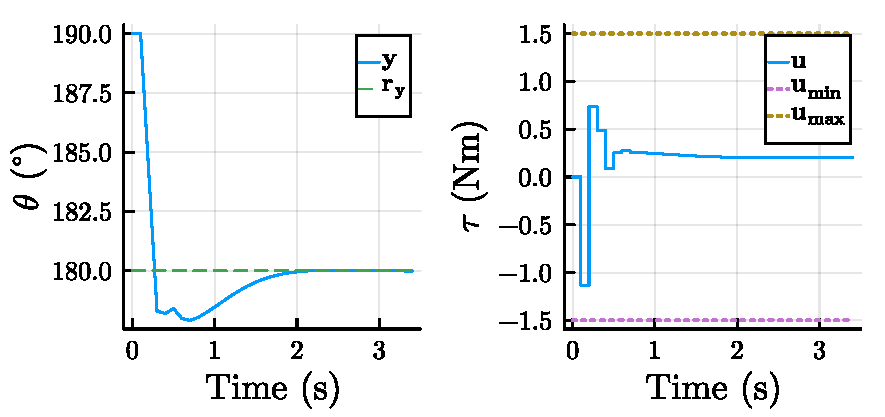
\includegraphics[width=0.5\columnwidth]{fig/plot_EconomMPC1.pdf}
    \label{fig:plot_EconomMPC1}
\end{figure}
\begin{figure}[ht]
    \centering
    \caption{Pendulum output disturbance rejection (EMPC).}
    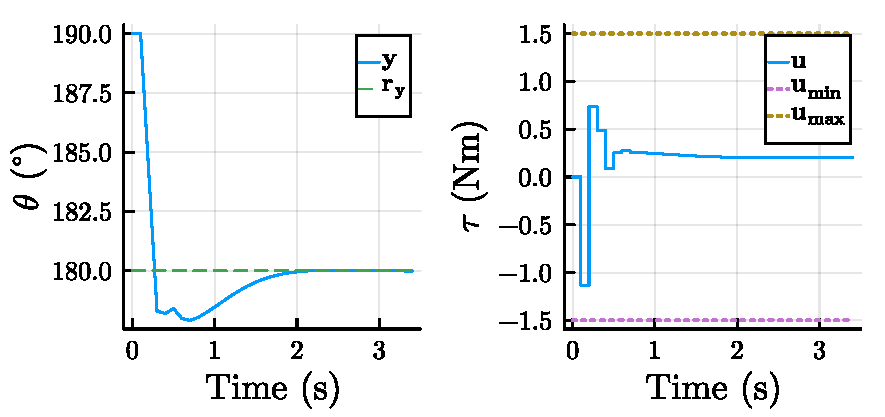
\includegraphics[width=0.5\columnwidth]{fig/plot_EconomMPC2.pdf}
    \label{fig:plot_EconomMPC2}
\end{figure}

\subsubsection{Successive Linearization Model Predictive Control (SLMPC)}
\label{sec:successive_linearization}

The \texttt{setmodel!} method allows online adaptation of a linear plant model. Combined with the automatic linearization of \texttt{linearize}, based on \texttt{ForwardDiff.jl}, a successive linearization MPC can be designed with minimal efforts. But first, the default \texttt{LinMPC} solver (\texttt{OSQP.jl}) does not perform as well as \texttt{DAQP.jl} on unstable plants like here \citep{daqp}. The syntax to install it is: 
\begin{minted}{julia}
using Pkg; Pkg.add(["JuMP","DAQP"]) # install JuMP and DAQP
using JuMP, DAQP
optim = JuMP.Model(DAQP.Optimizer, add_bridges=false)
\end{minted}
The bridges are a concept introduced by \texttt{JuMP.jl} to convert the constraints into a form that is natively supported by a specific solver (e.g.: from inequality to equality constraints). Disabling them slightly reduce the overhead when it is not required, like here. Next, the \texttt{SteadyKalmanFilter} does not support \texttt{setmodel!}, so we need to use the time-varying \texttt{KalmanFilter} instead:
\begin{minted}{julia}
linmodel = linearize(model, x=[0, 0], u=[0])
kf = KalmanFilter(linmodel; σQ, σR, nint_u, σQint_u)
mpc3 = LinMPC(kf; Hp, Hc, Mwt, Nwt, Cwt, optim)
mpc3 = setconstraint!(mpc3; umin, umax)
\end{minted}
\spacerepl
\begin{minted}{julia-repl}
LinMPC controller with a sample time Ts = 0.1 s, DAQP optimizer, KalmanFilter
estimator and:
 20 prediction steps Hp
  2 control steps Hc
  0 slack variable ϵ (control constraints)
  1 manipulated inputs u (1 integrating states)
  3 estimated states x̂
  1 measured outputs ym (0 integrating states)
  0 unmeasured outputs yu
  0 measured disturbances d
\end{minted}
A custom simulation function that successively linearizes the pendulum model and updates the \texttt{LinMPC} controller with \texttt{setmodel!} is required: 
\begin{minted}{julia}
function sim2!(mpc, nlmodel, N, ry, plant, x_0, x̂_0, y_step)
    U, Y, Ry = zeros(1, N), zeros(1, N), zeros(1, N)
    u, x̂ = [0], x̂_0
    initstate!(mpc, u, plant())
    setstate!(plant, x_0); setstate!(mpc, x̂_0)
    linmodel = linearize(nlmodel; u, x=x̂[1:2])
    setmodel!(mpc, linmodel)
    for i = 1:N
        y = plant() + y_step
        u = mpc(ry)
        linearize!(linmodel, nlmodel; u, x=x̂[1:2])
        setmodel!(mpc, linmodel) 
        U[:,i], Y[:,i], Ry[:,i] = u, y, ry
        x̂ = updatestate!(mpc, u, y)
        updatestate!(plant, u)
    end
    U_data, Y_data, Ry_data = U, Y, Ry
    return SimResult(mpc, U_data, Y_data; Ry_data)
end
\end{minted}
The new model is set after solving the optimization problem, and before updating the state estimate, that is, when both $\mathbf{u}(k)$ and $\mathbf{\hat{x}}_{k-1}(k)$ are available as the new operating point. As shown in \cref{fig:plot_SuccLinMPC1} and \ref{fig:plot_SuccLinMPC2}, the SLMPC closed-loop response is similar to the nonlinear MPC, both for the 180° setpoint:
\begin{minted}{julia}
x_0 = [0, 0]; x̂_0 = [0, 0, 0]; ry = [180]; y_step=[0]
res3_ry = sim2!(mpc3, model, N, ry, plant, x_0, x̂_0, y_step)
plot(res3_ry)
\end{minted}
and the 10° step disturbance:
\begin{minted}{julia}
x_0 = [π, 0]; x̂_0 = [π, 0, 0]; ry = [180]; y_step=[10]
res3_yd = sim2!(mpc3, model, N, ry, plant, x_0, x̂_0, y_step)
plot(res3_yd)
\end{minted}

\begin{figure}[ht]
    \centering
    \caption{Pendulum output setpoint tracking (SLMPC).}
    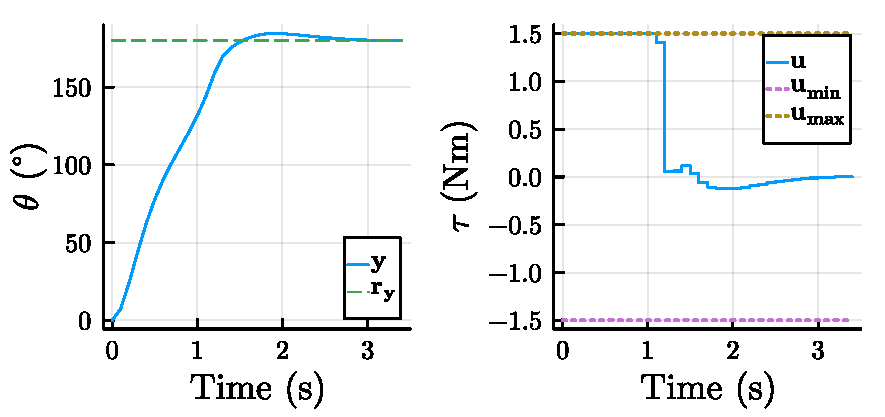
\includegraphics[width=0.5\columnwidth]{fig/plot_SuccLinMPC1.pdf}
    \label{fig:plot_SuccLinMPC1}
\end{figure}

\begin{figure}[ht]
    \centering
    \caption{Pendulum output disturbance rejection (SLMPC).}
    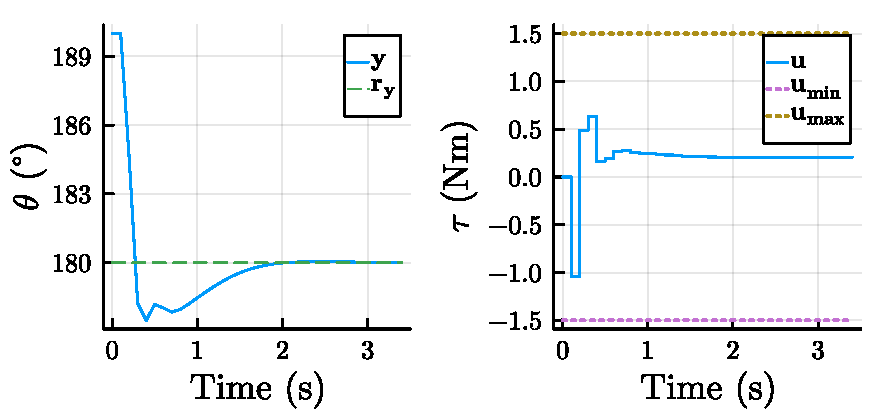
\includegraphics[width=0.5\columnwidth]{fig/plot_SuccLinMPC2.pdf}
    \label{fig:plot_SuccLinMPC2}
\end{figure}

The next section presents the interesting result: the solving time is drastically lower.

\subsection{Benchmarks}
\label{sec:benchmarks}

The time required to simulate the previous case studies is a benchmark of MPC performance in terms of computational cost (the cost to simulate the plant being negligible). The case studies are reproduced on MATLAB to compare the performance of the two frameworks. A special care is taken to ensure that that the closed-loop solution in MATLAB is identical to Julia’s counterpart. The median simulation time of 500 simulations, for MPC and SLMPC, and 50 simulations, for NMPC and EMPC, provide a performance benchmark robust to outliers. It must be emphasized that the reported values are the total time to simulate the whole scenario, that is $N=75$ time steps for the CSTR, and $N=35$, for the pendulum.

The MATLAB implementations use the model predictive control toolbox. Additional licenses to the control system and optimization toolboxes are needed to design and execute MPCs. Note that the SLMPC code relies on the symbolic toolbox, since there is no automatic differentiation in MATLAB. All the scripts are executed as is, in the interpreter. Code generation is typically required to produce fast dedicated code. But, as mentioned in the introduction, it creates other problems like extra licensing fees (e.g.: MATLAB/Simulink Coder). Also note that MATLAB only supports the less efficient non-mutating syntax for the nonlinear state-space functions.

Since the performance is solver-dependent, multiple optimization algorithms are tested. The results include four types of quadratic/nonlinear solvers. The operator-splitting (OS) methods are: 
\begin{itemize}
    \item \texttt{OSQP.jl} package in Julia \citep{osqp}
    \item \texttt{admm} option in MATLAB \citep{admm}
\end{itemize}
For active-set (AS) methods, the optimizers are: 
\begin{itemize}
    \item \texttt{DAQP.jl} package in Julia \citep{daqp}
    \item \texttt{active-set} option in MATLAB \citep{activeset}
\end{itemize}
For interior-point (IP) methods, the solvers are: 
\begin{itemize}
    \item \texttt{Ipopt.jl} package in Julia \citep{ipopt}
    \item \texttt{interior-point} option in MATLAB \citep{interiorpoint}
\end{itemize}
And, lastly, the sequential quadratic (SQ) methods are:
\begin{itemize}
    \item \texttt{KNITRO.jl} package in Julia \citep{knitro}
    \item \texttt{sqp} option in MATLAB \citep{sqp}
\end{itemize}

All the solvers in Julia are free and open-source, except for \texttt{KNITRO.jl} which is commercial. A separate keyword argument in the controller constructors allows customizing the solver (see \cref{sec:successive_linearization} for an example). Only the active-set results are include for the SLMPC since \texttt{OSQP.jl} does not work as well on the pendulum (without major modifications in the optimizer settings).

A laptop with an Intel\textsuperscript{\textregistered} Core\textsuperscript{\texttrademark} i7-1165G7 (8 cores at \SI{4.70}{\giga\hertz}) and a Linux v6.9.5 kernel runs the benchmarks. The scripts are executed on Julia v1.10.4 and MATLAB R2024a. A public repository at \url{https://github.com/franckgaga/mpcPackageJulia.tex} provides the code to reproduce the results. 

\begin{table}
    \centering
    \caption{Julia and MATLAB Benchmarks on the Case Studies.}
    \label{tab:benchamrks}
    \centering
    \small
    \begin{tabular}{llllrr}
	
\toprule %=======================================================================

	  &	& & & \multicolumn{2}{c}{Median Time (s)} \\ \cmidrule(l){5-6}
Plant & Control & Test & Solver & Julia & MATLAB \\
\midrule %--------------------------------------------------------------------

CSTR		& MPC	& W/O $\mathbf{d}$	& OS & \num{0.0013} & \num{0.0193}	\\
CSTR		& MPC	& W/O $\mathbf{d}$	& AS & \num{0.0043} & \num{0.0169}	\\
CSTR		& MPC	& With $\mathbf{d}$ & OS & \num{0.0013} & \num{0.0191}	\\
CSTR		& MPC	& With $\mathbf{d}$ & AS & \num{0.0043} & \num{0.0165}	\\
Pendulum 	& NMPC	& Track. 	   		& IP & \num{0.7023} & \num{1.3210}	\\
Pendulum 	& NMPC	& Track. 	   		& SQ & \num{0.2873} & \num{0.6391}	\\
Pendulum    & NMPC	& Regul. 			& IP & \num{0.6113} & \num{1.4252} 	\\
Pendulum    & NMPC	& Regul. 			& SQ & \num{0.2682} & \num{0.5701} 	\\
Pendulum    & EMPC	& Track.			& IP & \num{0.7195} & \num{1.0836} 	\\
Pendulum    & EMPC	& Track.			& SQ & \num{0.2999} & \num{0.7487} 	\\
Pendulum	& EMPC	& Regul. 			& IP & \num{0.6687} & \num{0.8575} 	\\
Pendulum	& EMPC	& Regul. 			& SQ & \num{0.2907} & \num{0.6717}  \\
	
\bottomrule %====================================================================
	
\end{tabular}
\end{table}

The benchmarks are presented in \cref{tab:benchamrks}. The linear MPC is significantly faster in Julia, approximately from 4 to 15 times faster. This result is however amplified by \texttt{OSQP.jl}, a modern and fast OS quadratic optimizer, which seems to perform considerably better than MATLAB's counterpart (\texttt{admm}). But the authors would argue that it is a consequence of \texttt{ModelPredictiveControl.jl} modular design. Any modern optimization tools can be leveraged with minimal effort and without any package update, presuming that they offer a \texttt{JuMP.jl} interface. Using a custom optimization algorithm in MATLAB MPC toolbox is possible but not straightforward.

The NMPC and EMPC are approximately twice as fast as MATLAB counterparts on average. This is presumably explained by MATLAB's internal and the pendulum model. Indeed, many built-in MATLAB functions are not purely interpreted but contains calls to specialized compiled code. This is probably the case for \texttt{fmincon} solvers, the function used by MATLAB NMPC toolset. And, since the pendulum model is trivially simple, computing the predictions is not a performance bottleneck. Thus, in both languages, the majority of the time is spent in the optimization algorithms, both implemented in machine code for most parts. It is expected that the speed gap between the two languages would be larger for more complex plant models, since this part is mainly interpreted in MATLAB. Lastly, SLMPC is about 4 times faster than MATLAB. It is also 75 times faster than the nonlinear controllers on average: an impressive gain for similar closed-loop response!